% Parent preamble: \usepackage{graphicx,amsmath,booktabs,multirow} (and caption if floats are customized).
\setlength{\belowcaptionskip}{6pt}
\section{Pseudopotential Kohn--Sham accuracy}

We next assess the accuracy of SPARC-atomSFE for pseudopotential Kohn--Sham DFT calculations through comparisons with the literature.
In particular, we compare against the spectral scheme based SPARC-atom code, implemented as part of the M-SPARC package, while considering four exchange-correlation functionals: LDA, PBE, rSCAN, and PBE0.
We compare the results for seven atoms spanning a range of chemical environments---$\mathrm{He}$, $\mathrm{N}$, $\mathrm{O}$, $\mathrm{Fe}$, $\mathrm{Mn}$, $\mathrm{Mo}$, and $\mathrm{Cs}$.
The distribution of the differences in the results is shown as violin plots in Figure~\ref{fig:psp-xc-accuracy-violin}.
We observe that total energies and occupied valence eigenvalues agree to $10^{-6}$~Ha or better for LDA, PBE, and rSCAN.
The exception is PBE0, which exhibits errors approximately an order of magnitude larger; this can be attributed to the fact that the quadrature in the spectral scheme used by SPARC-atom is limited to the degree of the polynomial used, making it difficult to converge calculations involving exact exchange, where higher-order quadrature is required.
This limitation can be overcome by adopting a differential approach for the exact exchange operator, as done in the present work.
These results demonstrate the accuracy of SPARC-atomSFE for atomic structure calculations based on pseudopotential Kohn--Sham DFT.

As supplementary material to the accuracy discussion above, we tabulate the full numerical data underlying Figure~\ref{fig:psp-xc-accuracy-violin} in Tables~\ref{tab:pseudo-lda-svwn-eigs}, \ref{tab:pseudo-gga-pbe-eigs}, \ref{tab:pseudo-rscan-eigs}, and~\ref{tab:pseudo-pbe0-eigs} (LDA-SVWN, GGA-PBE, rSCAN, and PBE0, respectively).

\begin{figure}[!htbp]
    \centering
    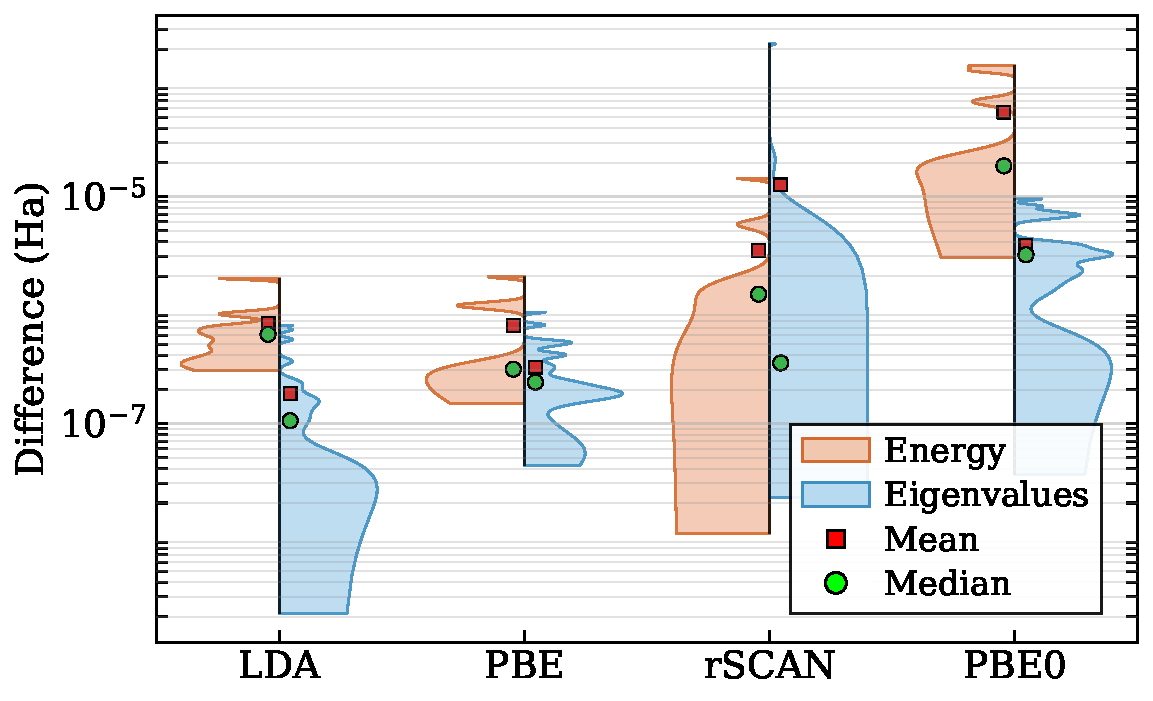
\includegraphics[width=\textwidth]{../figures/xc_accuracy_violin_psp}
    \caption{Comparison of SPARC-atomSFE pseudopotential Kohn--Sham DFT results with the M-SPARC SPARC-atom reference for various exchange-correlation functionals. The energy and eigenvalue errors denote the absolute differences in the corresponding quantities.}
    \label{fig:psp-xc-accuracy-violin}
\end{figure}


\begin{table}[!htbp]
    \centering
    \footnotesize
    \setlength{\tabcolsep}{3pt}
    \renewcommand{\arraystretch}{0.9}
    \caption{Comparison of the total energies and eigenvalues for the LDA-SVWN exchange-correlation functional based on norm-conserving pseudopotential atomic calculations.}
    \label{tab:pseudo-lda-svwn-eigs}
    \begin{tabular}{@{}l c ccc ccc ccc@{}}
        \toprule
        & & \multicolumn{3}{c}{$-E_{\mathrm{tot}}$ (Ha)} & \multicolumn{6}{c}{$-\varepsilon_{nl}$ (Ha)} \\
        \cmidrule(lr){3-5} \cmidrule(lr){6-11}
         & $Z$ & atomSFE & M-SPARC & Difference & $n$ & $\ell$ & $g_{nl}$ & atomSFE & M-SPARC & Difference \\
        \midrule
        \multirow[t]{1}{*}{He} & \multirow[t]{1}{*}{2} & \multirow[t]{1}{*}{$2.800084291$} & \multirow[t]{1}{*}{$2.800083994$} & \multirow[t]{1}{*}{$2.97 \times 10^{-7}$} & 1 & 0 & 2 & $0.57046$ & $0.57046$ & $1.52 \times 10^{-7}$ \\
        \multirow[t]{2}{*}{N} & \multirow[t]{2}{*}{7} & \multirow[t]{2}{*}{$10.0228671$} & \multirow[t]{2}{*}{$10.02286518$} & \multirow[t]{2}{*}{$1.91 \times 10^{-6}$} & 2 & 0 & 2 & $0.67708$ & $0.677081$ & $6.72 \times 10^{-7}$ \\
         &  &  &  &  & 2 & 1 & 3 & $0.266124$ & $0.266124$ & $5.53 \times 10^{-7}$ \\
        \multirow[t]{2}{*}{O} & \multirow[t]{2}{*}{8} & \multirow[t]{2}{*}{$16.21748133$} & \multirow[t]{2}{*}{$16.21748084$} & \multirow[t]{2}{*}{$4.91 \times 10^{-7}$} & 2 & 0 & 2 & $0.873064$ & $0.873065$ & $7.37 \times 10^{-7}$ \\
         &  &  &  &  & 2 & 1 & 4 & $0.338133$ & $0.338133$ & $3.56 \times 10^{-7}$ \\
        \multirow[t]{4}{*}{Mn} & \multirow[t]{4}{*}{25} & \multirow[t]{4}{*}{$105.2337256$} & \multirow[t]{4}{*}{$105.2337263$} & \multirow[t]{4}{*}{$7.14 \times 10^{-7}$} & 3 & 0 & 2 & $3.138755$ & $3.138755$ & $4.54 \times 10^{-8}$ \\
         &  &  &  &  & 3 & 1 & 6 & $2.002629$ & $2.002629$ & $3.21 \times 10^{-9}$ \\
         &  &  &  &  & 3 & 2 & 5 & $0.257732$ & $0.257732$ & $2.12 \times 10^{-7}$ \\
         &  &  &  &  & 4 & 0 & 2 & $0.194097$ & $0.194097$ & $1.39 \times 10^{-8}$ \\
        \multirow[t]{4}{*}{Fe} & \multirow[t]{4}{*}{26} & \multirow[t]{4}{*}{$116.7411744$} & \multirow[t]{4}{*}{$116.741174$} & \multirow[t]{4}{*}{$3.69 \times 10^{-7}$} & 3 & 0 & 2 & $3.436694$ & $3.436694$ & $3.18 \times 10^{-8}$ \\
         &  &  &  &  & 3 & 1 & 6 & $2.202574$ & $2.202574$ & $2.82 \times 10^{-8}$ \\
         &  &  &  &  & 3 & 2 & 6 & $0.285108$ & $0.285108$ & $2.5 \times 10^{-8}$ \\
         &  &  &  &  & 4 & 0 & 2 & $0.201428$ & $0.201428$ & $3.84 \times 10^{-8}$ \\
        \multirow[t]{4}{*}{Mo} & \multirow[t]{4}{*}{42} & \multirow[t]{4}{*}{$69.69080029$} & \multirow[t]{4}{*}{$69.69080091$} & \multirow[t]{4}{*}{$6.14 \times 10^{-7}$} & 4 & 0 & 2 & $2.367637$ & $2.367637$ & $1.04 \times 10^{-7}$ \\
         &  &  &  &  & 4 & 1 & 6 & $1.418245$ & $1.418244$ & $1.7 \times 10^{-7}$ \\
         &  &  &  &  & 4 & 2 & 5 & $0.144562$ & $0.144562$ & $1.09 \times 10^{-7}$ \\
         &  &  &  &  & 5 & 0 & 1 & $0.158758$ & $0.158758$ & $3.55 \times 10^{-8}$ \\
        \multirow[t]{3}{*}{Cs} & \multirow[t]{3}{*}{55} & \multirow[t]{3}{*}{$23.31026826$} & \multirow[t]{3}{*}{$23.31026919$} & \multirow[t]{3}{*}{$9.25 \times 10^{-7}$} & 5 & 0 & 2 & $0.988689$ & $0.988689$ & $2.37 \times 10^{-7}$ \\
         &  &  &  &  & 5 & 1 & 6 & $0.500169$ & $0.500169$ & $1.55 \times 10^{-7}$ \\
         &  &  &  &  & 6 & 0 & 1 & $0.081715$ & $0.081715$ & $2.11 \times 10^{-9}$ \\
        \bottomrule
    \end{tabular}
\end{table}

\begin{table}[!htbp]
    \centering
    \footnotesize
    \setlength{\tabcolsep}{3pt}
    \renewcommand{\arraystretch}{0.9}
    \caption{Comparison of the total energies and eigenvalues for the GGA-PBE exchange-correlation functional based on norm-conserving pseudopotential atomic calculations.}
    \label{tab:pseudo-gga-pbe-eigs}
    \begin{tabular}{@{}l c ccc ccc ccc@{}}
        \toprule
        & & \multicolumn{3}{c}{$-E_{\mathrm{tot}}$ (Ha)} & \multicolumn{6}{c}{$-\varepsilon_{nl}$ (Ha)} \\
        \cmidrule(lr){3-5} \cmidrule(lr){6-11}
         & $Z$ & atomSFE & M-SPARC & Difference & $n$ & $\ell$ & $g_{nl}$ & atomSFE & M-SPARC & Difference \\
        \midrule
        \multirow[t]{1}{*}{He} & \multirow[t]{1}{*}{2} & \multirow[t]{1}{*}{$2.853330662$} & \multirow[t]{1}{*}{$2.853330926$} & \multirow[t]{1}{*}{$2.64 \times 10^{-7}$} & 1 & 0 & 2 & $0.579311$ & $0.579311$ & $2.35 \times 10^{-7}$ \\
        \multirow[t]{2}{*}{N} & \multirow[t]{2}{*}{7} & \multirow[t]{2}{*}{$10.05930315$} & \multirow[t]{2}{*}{$10.05930012$} & \multirow[t]{2}{*}{$3.03 \times 10^{-6}$} & 2 & 0 & 2 & $0.682914$ & $0.682914$ & $3.92 \times 10^{-7}$ \\
         &  &  &  &  & 2 & 1 & 3 & $0.260551$ & $0.260551$ & $6.63 \times 10^{-7}$ \\
        \multirow[t]{2}{*}{O} & \multirow[t]{2}{*}{8} & \multirow[t]{2}{*}{$16.27370467$} & \multirow[t]{2}{*}{$16.27370633$} & \multirow[t]{2}{*}{$1.66 \times 10^{-6}$} & 2 & 0 & 2 & $0.880576$ & $0.880576$ & $6.52 \times 10^{-7}$ \\
         &  &  &  &  & 2 & 1 & 4 & $0.331872$ & $0.331872$ & $2.07 \times 10^{-7}$ \\
        \multirow[t]{4}{*}{Mn} & \multirow[t]{4}{*}{25} & \multirow[t]{4}{*}{$105.3660140$} & \multirow[t]{4}{*}{$105.3660158$} & \multirow[t]{4}{*}{$1.83 \times 10^{-6}$} & 3 & 0 & 2 & $3.156010$ & $3.156010$ & $1.38 \times 10^{-7}$ \\
         &  &  &  &  & 3 & 1 & 6 & $2.006265$ & $2.006265$ & $9.34 \times 10^{-8}$ \\
         &  &  &  &  & 3 & 2 & 5 & $0.248834$ & $0.248834$ & $3.64 \times 10^{-7}$ \\
         &  &  &  &  & 4 & 0 & 2 & $0.187686$ & $0.187687$ & $4.18 \times 10^{-7}$ \\
        \multirow[t]{4}{*}{Fe} & \multirow[t]{4}{*}{26} & \multirow[t]{4}{*}{$116.7788402$} & \multirow[t]{4}{*}{$116.7788403$} & \multirow[t]{4}{*}{$9.29 \times 10^{-8}$} & 3 & 0 & 2 & $3.455077$ & $3.455077$ & $1.76 \times 10^{-9}$ \\
         &  &  &  &  & 3 & 1 & 6 & $2.206535$ & $2.206535$ & $8.20 \times 10^{-8}$ \\
         &  &  &  &  & 3 & 2 & 6 & $0.275801$ & $0.275801$ & $3.47 \times 10^{-9}$ \\
         &  &  &  &  & 4 & 0 & 2 & $0.194482$ & $0.194482$ & $2.37 \times 10^{-8}$ \\
        \multirow[t]{4}{*}{Mo} & \multirow[t]{4}{*}{42} & \multirow[t]{4}{*}{$69.67943092$} & \multirow[t]{4}{*}{$69.67942912$} & \multirow[t]{4}{*}{$1.79 \times 10^{-6}$} & 4 & 0 & 2 & $2.364713$ & $2.364713$ & $1.15 \times 10^{-7}$ \\
         &  &  &  &  & 4 & 1 & 6 & $1.414321$ & $1.414321$ & $1.21 \times 10^{-8}$ \\
         &  &  &  &  & 4 & 2 & 5 & $0.137922$ & $0.137922$ & $1.82 \times 10^{-7}$ \\
         &  &  &  &  & 5 & 0 & 1 & $0.150181$ & $0.150181$ & $4.06 \times 10^{-8}$ \\
        \multirow[t]{3}{*}{Cs} & \multirow[t]{3}{*}{55} & \multirow[t]{3}{*}{$23.24984140$} & \multirow[t]{3}{*}{$23.24984231$} & \multirow[t]{3}{*}{$9.15 \times 10^{-7}$} & 5 & 0 & 2 & $0.982389$ & $0.982389$ & $7.55 \times 10^{-8}$ \\
         &  &  &  &  & 5 & 1 & 6 & $0.496788$ & $0.496788$ & $1.59 \times 10^{-7}$ \\
         &  &  &  &  & 6 & 0 & 1 & $0.076670$ & $0.076669$ & $3.29 \times 10^{-8}$ \\
        \bottomrule
    \end{tabular}
\end{table}

\begin{table}[!htbp]
    \centering
    \footnotesize
    \setlength{\tabcolsep}{3pt}
    \renewcommand{\arraystretch}{0.9}
    \caption{Comparison of the total energies and eigenvalues for the rSCAN exchange-correlation functional based on norm-conserving pseudopotential atomic calculations.}
    \label{tab:pseudo-rscan-eigs}
    \begin{tabular}{@{}l c ccc ccc ccc@{}}
        \toprule
        & & \multicolumn{3}{c}{$-E_{\mathrm{tot}}$ (Ha)} & \multicolumn{6}{c}{$-\varepsilon_{nl}$ (Ha)} \\
        \cmidrule(lr){3-5} \cmidrule(lr){6-11}
         & $Z$ & atomSFE & M-SPARC & Difference & $n$ & $\ell$ & $g_{nl}$ & atomSFE & M-SPARC & Difference \\
        \midrule
        \multirow[t]{1}{*}{He} & \multirow[t]{1}{*}{2} & \multirow[t]{1}{*}{$2.803317365$} & \multirow[t]{1}{*}{$2.803317354$} & \multirow[t]{1}{*}{$1.07 \times 10^{-8}$} & 1 & 0 & 2 & $0.605361$ & $0.605361$ & $6.61 \times 10^{-8}$ \\
        \multirow[t]{2}{*}{N} & \multirow[t]{2}{*}{7} & \multirow[t]{2}{*}{$9.620390181$} & \multirow[t]{2}{*}{$9.620390518$} & \multirow[t]{2}{*}{$3.37 \times 10^{-7}$} & 2 & 0 & 2 & $0.729363$ & $0.729363$ & $1.45 \times 10^{-7}$ \\
         &  &  &  &  & 2 & 1 & 3 & $0.26564$ & $0.265639$ & $3.03 \times 10^{-7}$ \\
        \multirow[t]{2}{*}{O} & \multirow[t]{2}{*}{8} & \multirow[t]{2}{*}{$15.70167901$} & \multirow[t]{2}{*}{$15.70168048$} & \multirow[t]{2}{*}{$1.47 \times 10^{-6}$} & 2 & 0 & 2 & $0.940105$ & $0.940105$ & $5.79 \times 10^{-7}$ \\
         &  &  &  &  & 2 & 1 & 4 & $0.343355$ & $0.343355$ & $4.7 \times 10^{-8}$ \\
        \multirow[t]{4}{*}{Mn} & \multirow[t]{4}{*}{25} & \multirow[t]{4}{*}{$99.17611481$} & \multirow[t]{4}{*}{$99.17611343$} & \multirow[t]{4}{*}{$1.38 \times 10^{-6}$} & 3 & 0 & 2 & $3.279161$ & $3.279161$ & $3.62 \times 10^{-7}$ \\
         &  &  &  &  & 3 & 1 & 6 & $2.08522$ & $2.085219$ & $3.09 \times 10^{-7}$ \\
         &  &  &  &  & 3 & 2 & 5 & $0.251825$ & $0.251825$ & $3.86 \times 10^{-7}$ \\
         &  &  &  &  & 4 & 0 & 2 & $0.195917$ & $0.195917$ & $2.25 \times 10^{-8}$ \\
        \multirow[t]{4}{*}{Fe} & \multirow[t]{4}{*}{26} & \multirow[t]{4}{*}{$118.0039187$} & \multirow[t]{4}{*}{$118.003913$} & \multirow[t]{4}{*}{$5.71 \times 10^{-6}$} & 3 & 0 & 2 & $3.585989$ & $3.585987$ & $2.53 \times 10^{-6}$ \\
         &  &  &  &  & 3 & 1 & 6 & $2.293534$ & $2.293532$ & $2.09 \times 10^{-6}$ \\
         &  &  &  &  & 3 & 2 & 6 & $0.281913$ & $0.281911$ & $1.65 \times 10^{-6}$ \\
         &  &  &  &  & 4 & 0 & 2 & $0.203008$ & $0.203008$ & $6.33 \times 10^{-7}$ \\
        \multirow[t]{4}{*}{Mo} & \multirow[t]{4}{*}{42} & \multirow[t]{4}{*}{$68.16700484$} & \multirow[t]{4}{*}{$68.16700474$} & \multirow[t]{4}{*}{$9.92 \times 10^{-8}$} & 4 & 0 & 2 & $2.45666$ & $2.456659$ & $3.86 \times 10^{-7}$ \\
         &  &  &  &  & 4 & 1 & 6 & $1.469806$ & $1.469806$ & $3.24 \times 10^{-7}$ \\
         &  &  &  &  & 4 & 2 & 5 & $0.13904$ & $0.13904$ & $2.88 \times 10^{-7}$ \\
         &  &  &  &  & 5 & 0 & 1 & $0.154164$ & $0.154164$ & $7.69 \times 10^{-8}$ \\
        \multirow[t]{3}{*}{Cs} & \multirow[t]{3}{*}{55} & \multirow[t]{3}{*}{$20.17964157$} & \multirow[t]{3}{*}{$20.17965618$} & \multirow[t]{3}{*}{$1.46 \times 10^{-5}$} & 5 & 0 & 2 & $1.023347$ & $1.023124$ & $2.23 \times 10^{-4}$ \\
         &  &  &  &  & 5 & 1 & 6 & $0.51887$ & $0.51887$ & $1.72 \times 10^{-7}$ \\
         &  &  &  &  & 6 & 0 & 1 & $0.076458$ & $0.076437$ & $2.12 \times 10^{-5}$ \\
        \bottomrule
    \end{tabular}
\end{table}

\begin{table}[!htbp]
    \centering
    \footnotesize
    \setlength{\tabcolsep}{3pt}
    \renewcommand{\arraystretch}{0.9}
    \caption{Comparison of the total energies and eigenvalues for the PBE0 exchange-correlation functional based on norm-conserving pseudopotential atomic calculations.}
    \label{tab:pseudo-pbe0-eigs}
    \begin{tabular}{@{}l c ccc ccc ccc@{}}
        \toprule
        & & \multicolumn{3}{c}{$-E_{\mathrm{tot}}$ (Ha)} & \multicolumn{6}{c}{$-\varepsilon_{nl}$ (Ha)} \\
        \cmidrule(lr){3-5} \cmidrule(lr){6-11}
         & $Z$ & atomSFE & M-SPARC & Difference & $n$ & $\ell$ & $g_{nl}$ & atomSFE & M-SPARC & Difference \\
        \midrule
        \multirow[t]{1}{*}{He} & \multirow[t]{1}{*}{2} & \multirow[t]{1}{*}{$2.858444072$} & \multirow[t]{1}{*}{$2.858447011$} & \multirow[t]{1}{*}{$2.94 \times 10^{-6}$} & 1 & 0 & 2 & $0.668803$ & $0.668805$ & $1.88 \times 10^{-6}$ \\
        \multirow[t]{2}{*}{N} & \multirow[t]{2}{*}{7} & \multirow[t]{2}{*}{$9.8409288$} & \multirow[t]{2}{*}{$9.840936922$} & \multirow[t]{2}{*}{$8.12 \times 10^{-6}$} & 2 & 0 & 2 & $0.781191$ & $0.781194$ & $3.11 \times 10^{-6}$ \\
         &  &  &  &  & 2 & 1 & 3 & $0.268917$ & $0.268919$ & $1.45 \times 10^{-6}$ \\
        \multirow[t]{2}{*}{O} & \multirow[t]{2}{*}{8} & \multirow[t]{2}{*}{$16.01035357$} & \multirow[t]{2}{*}{$16.01037228$} & \multirow[t]{2}{*}{$1.87 \times 10^{-5}$} & 2 & 0 & 2 & $0.999295$ & $0.999299$ & $3.78 \times 10^{-6}$ \\
         &  &  &  &  & 2 & 1 & 4 & $0.36414$ & $0.364142$ & $2.37 \times 10^{-6}$ \\
        \multirow[t]{4}{*}{Mn} & \multirow[t]{4}{*}{25} & \multirow[t]{4}{*}{$103.7537001$} & \multirow[t]{4}{*}{$103.7538296$} & \multirow[t]{4}{*}{$1.3 \times 10^{-4}$} & 3 & 0 & 2 & $3.363098$ & $3.363104$ & $6.43 \times 10^{-6}$ \\
         &  &  &  &  & 3 & 1 & 6 & $2.162649$ & $2.162657$ & $8.26 \times 10^{-6}$ \\
         &  &  &  &  & 3 & 2 & 5 & $0.258815$ & $0.258822$ & $6.89 \times 10^{-6}$ \\
         &  &  &  &  & 4 & 0 & 2 & $0.214786$ & $0.214786$ & $4.08 \times 10^{-7}$ \\
        \multirow[t]{4}{*}{Fe} & \multirow[t]{4}{*}{26} & \multirow[t]{4}{*}{$115.7186491$} & \multirow[t]{4}{*}{$115.718792$} & \multirow[t]{4}{*}{$1.43 \times 10^{-4}$} & 3 & 0 & 2 & $3.665564$ & $3.665571$ & $6.96 \times 10^{-6}$ \\
         &  &  &  &  & 3 & 1 & 6 & $2.363997$ & $2.364006$ & $9.61 \times 10^{-6}$ \\
         &  &  &  &  & 3 & 2 & 6 & $0.298827$ & $0.298834$ & $7.47 \times 10^{-6}$ \\
         &  &  &  &  & 4 & 0 & 2 & $0.222093$ & $0.222093$ & $3.07 \times 10^{-7}$ \\
        \multirow[t]{4}{*}{Mo} & \multirow[t]{4}{*}{42} & \multirow[t]{4}{*}{$68.96799747$} & \multirow[t]{4}{*}{$68.96806647$} & \multirow[t]{4}{*}{$6.9 \times 10^{-5}$} & 4 & 0 & 2 & $2.526861$ & $2.526864$ & $3.36 \times 10^{-6}$ \\
         &  &  &  &  & 4 & 1 & 6 & $1.53111$ & $1.531114$ & $3.84 \times 10^{-6}$ \\
         &  &  &  &  & 4 & 2 & 5 & $0.144336$ & $0.144338$ & $2.22 \times 10^{-6}$ \\
         &  &  &  &  & 5 & 0 & 1 & $0.147808$ & $0.147807$ & $3.82 \times 10^{-7}$ \\
        \multirow[t]{3}{*}{Cs} & \multirow[t]{3}{*}{55} & \multirow[t]{3}{*}{$22.42005527$} & \multirow[t]{3}{*}{$22.42007389$} & \multirow[t]{3}{*}{$1.86 \times 10^{-5}$} & 5 & 0 & 2 & $1.066609$ & $1.066612$ & $2.9 \times 10^{-6}$ \\
         &  &  &  &  & 5 & 1 & 6 & $0.551291$ & $0.551294$ & $3.06 \times 10^{-6}$ \\
         &  &  &  &  & 6 & 0 & 1 & $0.076059$ & $0.076059$ & $3.59 \times 10^{-8}$ \\
        \bottomrule
    \end{tabular}
\end{table}
